\documentclass{article}
\usepackage{graphicx}
\usepackage{subcaption}

\begin{document}
	\begin{figure}[h!]
		\centering
		\begin{subfigure}[b]{0.3\linewidth}
			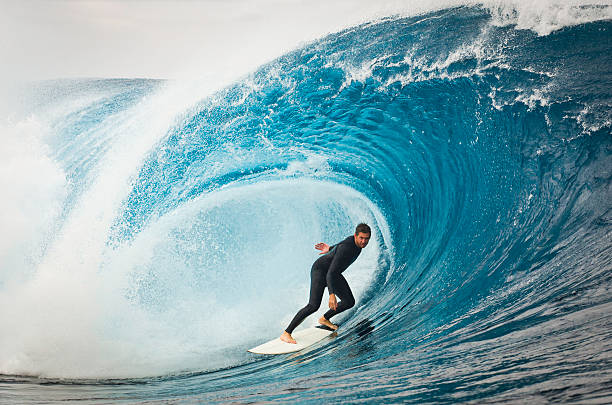
\includegraphics[width=\linewidth]{surf.jpg}
			\caption{surfing.}
		\end{subfigure}
		\begin{subfigure}[b]{0.3\linewidth}
			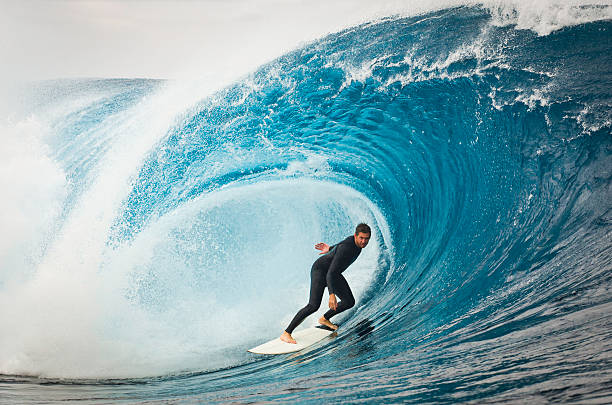
\includegraphics[width=\linewidth]{surf.jpg}
			\caption{Some more surfing}
		\end{subfigure}
		\begin{subfigure}[b]{0.3\linewidth}
			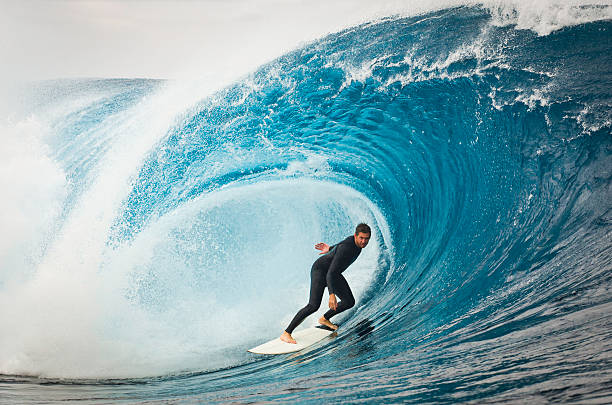
\includegraphics[width=\linewidth]{surf.jpg}
			\caption{even more surfing}
		\end{subfigure}
		\begin{subfigure}[b]{0.5\linewidth}
			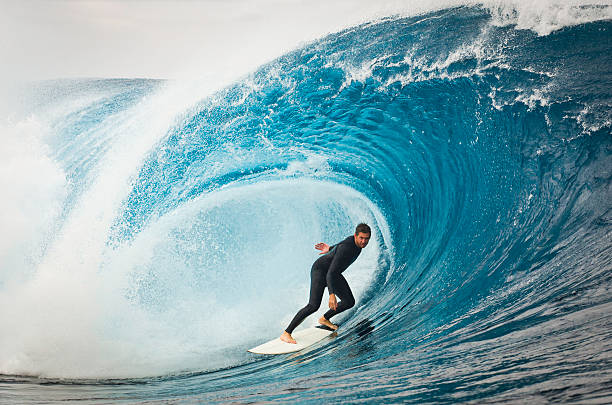
\includegraphics[width=\linewidth]{surf.jpg}
			\caption{Now that's alot of surfing.}
		\end{subfigure}
		\caption{The same man surfing multiple times.}
		\label{fig:surf}
	\end{figure}
\end{document}